%%%%                          %%%%
%%%% FUNDAMENTOS TECNOLÓGICOS %%%%
%%%%                          %%%%

\chapter{Fundamentos tecnológicos}
\label{chap:fundamentos-tecnologicos}

El objetivo de este capítulo es sentar las bases tecnológicas y teóricas sobre las que se ha llevado a cabo el proyecto.

\section{El formato PDF}

PDF es un formato digital para la creación de documentos introducido por Adobe Systems en 1993 \cite{adobe_systems_inc_quick_2010}. En los siguientes años el uso de este formato se extendió por toda la sociedad tanto en el ámbito público como privado. En el año 2008 la ISO publicó el estándar 32000-1 a partir de la versión 1.7 liberada por Adobe \cite{adobe_systems_inc_iso_2008}. Con posterioridad se publicó la versión 2.0 como ISO 32000-2 \cite{international_organization_for_standardization_iso_2017} en el año 2017 y una actualización en el 2020. PDF es un modelo de representación de imágenes que deriva del lenguaje PostScript para descripción de páginas. El modelo de imagen admite gráficos y texto de forma independiente al dispositivo de salida.

\subsection{Estructura de un PDF}

Un PDF no es un documento de texto, es un fichero binario de 8 bits que posee cierta estructura. El formato soporta varios tipos de datos para la representación de la información. Entre ellos está el formato \verb|String| que se utiliza para representar texto. También hay arrays, diccionarios (tablas asociativas con pares clave/valor) y tipo más básicos como booleanos, enteros o reales. Con estos tipos de datos se construyen objetos que son los que finalmente almacenan la información que se visualiza.

A nivel estructura física, un PDF tiene cuatro regiones. En orden secuencial están, la cabecera, que indica que se trata de un PDF y versión del estándar utilizado. El cuerpo que almacena todos los objetos definidos. Después está la Tabla de Referencias Cruzadas que se utiliza para la navegación y/o avance por el documento. En la tabla están los valores de desplazamiento para todos los objetos indirectos del documento. El cuarto elemento es el \verb|trailer|. Contiene varias claves, las más importantes son \verb|Size| que informa del número de entradas en la Tabla de Referencias Cruzadas y \verb|Root| que apunta al Catálogo del documento, lugar de comienzo de los objetos.

\subsection{Extracción de datos desde PDF}

\begin{itemize}
    \item Hablar de pdftotext
    \item PDFBox
\end{itemize}

\section{Información de coordenadas en documentos}

La base de este proyecto consiste en utilizar las coordenadas físicas de los textos existentes en los documentos. Dado que los PDF pueden contener una representación textual o simplemente imágenes por cada página, es necesario encontrar una solución aplicable a cada caso y que permita un tratamiento homogéneo en los sucesivos pasos.

\subsection{El microformato hOCR y otras alternativas}

HOCR es un microformato para la representación de la información de salida del proceso OCR. Los microformatos permiten dotar de datos estructurados a 

\subsection{Pdftotext e información de bounding box}

\verb|pdftotext| es una herramienta que permite extraer el texto contenido en un PDF. Existen otras herramientas similares, por ejemplo Apache PDFBox \cite{the_apache_software_foundation_apache_nodate}, pero durante el desarrollo \verb|pdftotext| fue la que mostró los resultados más útiles para los objetivos del proyecto. La implementación original de esta utilidad fue realizada por Glyph \& Cog \cite{glyph__cog_llc_glyph_nodate-1} junto con otras herramientas para tratamiento del formato PDF. En el año 2005 nace la librería Poppler a partir del \emph{fork} de la versión 3.0.3 del visor de \verb|xpdf| \cite{kristian_hogsberg_poppler_2012}. La implementación de Poppler está disponible por defecto en las principales distribuciones Linux. Además del extractor de texto, el proyecto tienen otras utilidades para tratamiento de PDF, por ejemplo, separación y unión de páginas, obtención de imágenes, etc.

La salida con la información de coordenadas, o bounding box, además del texto existe gracias a una aportación al proyecto del año 2010 de Kenneth Berland \cite{kenneth_berland_poppler_2010}. La información se proporciona en formato XHTML y se identifican \emph{tags} para bloques, lineas y palabras. En cada uno se informa de la localización del rectángulo que engloba al elemento con cuatro valores: \emph{xMin}, \emph{xMax}, \emph{yMin}, \emph{yMax}.

%% Incluir imagen del rectángulo
\begin{figure}[hp!]
	\centering
	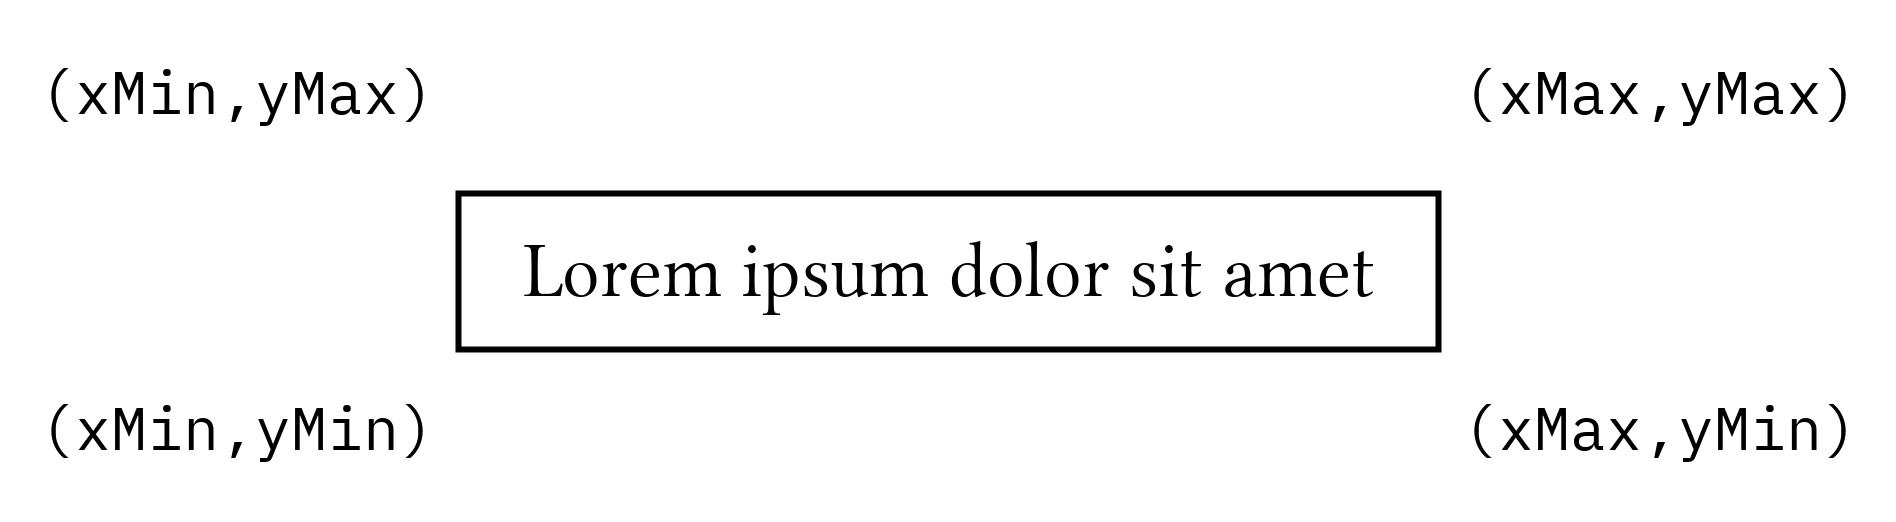
\includegraphics[width=0.75\textwidth]{imaxes/c-fundamentos-techno/correspondencia-coordenadas-bounding.png}
	\caption{Correspondencia de las coordenadas en una bounding box}
	\label{fig:bounding-box}
\end{figure}

\section{OCR con Tesseract}

Existen numerosas herramientas para llevar a cabo Reconocimiento Óptico de Caracteres. Entre ellas destaca Tesseract. Tesseract es un \emph{engine} de código abierto y desarrollado inicialmente por Hewlett Packard entre los años 1985 y 1995. Después de un periodo sin actividad, en el 2006 el proyecto fue recuperado por Google, que lo mantiene desde entonces.

Hoy en día tiene soporte para más de cien idiomas y la red neuronal que utiliza \footnote{Desde la versión 4, Tesseract utiliza una red LSTM. Esta es una red neuronal de tipo recurrente o RNN} puede ser entrenada para casos específicos si fuese necesario. Existe una amplia documentación en la web oficial, además, numerosos tutoriales en la red permiten familiarizarse con la herramienta al tratarse de un proyecto bien conocido y de larga trayectoria.

Se puede obtener como salida el texto reconocido y también la información de las coordenada, sobre el documento, de las palabras detectadas. Esta información resulta fundamental para poder aplicar las plantillas utilizadas este proyecto.

\section{Transformada de Hough}

La transformada de Hough es una técnica de visión por computador utilizada para detectar figuras parametrizables, tales como líneas o círculos. El algoritmo parte de una imagen binaria que representa los bordes encontrados por una detector de bordes. A continuación se calculan todas las posibles líneas que podrían pasar por cada punto y se lleva a cabo una votación. Se seleccionan las líneas más votadas, entre todas las detectadas.

Este algoritmo proporciona una manera automática de localizar los bordes entre líneas de las tablas de muchos documentos y evita la necesidad de incorporar dicha información a las plantillas de forma manual. Se utiliza la implementación incluida en la librería OpenCV.

\section{GNU Make}

GNU Make es una herramienta que permite automatizar transformaciones sobre ficheros. \verb|make| es capaz de construir ejecutables a partir del código fuente de un proyecto. Para ello utiliza un fichero \verb|makefile| que contiene todas las reglas necesarias.

\section{Flex y Bison}

Flex y Bison son dos herramientas utilizadas en conjunto para construir analizadores sintácticos. ¿Qué es un analizador sintáctico?

La primera se utiliza para crear escáneres y la segunda para generar parsers. Ambas utilizan como entrada unos ficheros que definen las reglas válidas.

\section{Ansible}



\section{Docker}




%% Valorar si mencionar otras herramientas como:
% Extracción de texto: , pdftotext
% Pretty print de JSON: jq
